\documentclass[a4paper,11pt]{article}

%%%%%%%%%
%%usees%%
%%%%%%%%%
\usepackage[utf8]{inputenc}
%\usepackage[ngerman]{babel}
%\usepackage{a4wide}
\usepackage[margin=3.0cm, top=3.0cm, bottom=3.0cm]{geometry}
\usepackage{setspace}
\usepackage{graphicx}
\usepackage{amssymb} 
\usepackage{amsmath}
\usepackage{mathtools}
\usepackage{footnote}
\usepackage{caption}
\usepackage{color}
\usepackage[hidelinks]{hyperref}
\usepackage{cite}
\usepackage{todonotes}
\usepackage{subfigure}
\usepackage{siunitx}
\usepackage{tabularx}
\usepackage{wrapfig}
\usepackage{url}
\usepackage{listings}


\newcommand{\reffig}[1]{Figure~\ref{#1}}
\newcommand{\refsec}[1]{Section~\ref{#1}}
\newcommand{\refdef}[1]{Definition~\ref{#1}}
\newcommand{\reflst}[1]{Listing~\ref{#1}}
\newcommand{\reftab}[1]{Table~\ref{#1}}

\definecolor{Mulberry}{cmyk}{0.34,0.90,0,0.02}
\definecolor{BrickRed}{cmyk}{0,0.89,0.94,0.28}
\lstset{language=C++,frame=none, basicstyle=\tt}
\lstdefinelanguage{CLIPS}{
  keywordsprefix=?,
  %keywordsprefix=\$,
  alsoletter={?=-<>*\$},
  keywordstyle=\color{Mulberry!80!black}\bfseries,
  keywords=[2]{deffunction, deftemplate, defrule, deffacts, defgeneric,
    defmodule, defadvice, defglobal, defmethod, definstance, defclass},
  keywordstyle=[2]\color{BrickRed!70!blue}\bfseries,
  keywords=[3]{slot, multislot, type, default, default-dynamic,
                      extends, crlf, range, nil, if, then, else, while,
                      not, or, switch, case, and, reset,
                      assert, test, declare, salience, return, bind, modify,
                      retract, explicit, unique, node-index-hash,
                      halt, printout, =>, <-},
  keywordstyle=[3]\color{darkgray}\bfseries,
  keywords=[4]{subsetp,progn, progn$, not, node-index-hash, create$,
    append$, length$, printout},%
  keywordstyle=[4]\color{gray}\bfseries,
  %identifierstyle=\color{black},
  sensitive=false,
  comment=[l]{;},
  commentstyle=\color{purple}\ttfamily,
  stringstyle=\color{red}\ttfamily,
  morestring=[b]"
}


\lstdefinestyle{CLIPS}
{
  language=CLIPS,
  basicstyle=\footnotesize\ttfamily\vspace{0.2cm},
  breaklines=true,
  showstringspaces=false,
  %keywordstyle=\bfseries,
  %keywordstyle=\color{Mulberry},
  frame=lines,
  belowcaptionskip=-3pt,
  emphstyle=\itshape,
  numbers=left,
  stepnumber=1,
  backgroundcolor=\color{gray!10},
  rulecolor=\color{gray!80},
  fillcolor=\color{gray!10},
  framexleftmargin=16pt,
  xleftmargin=16pt,
  %stringstyle=\color{BitterSweet},
  stringstyle=\color{BrickRed},
  commentstyle=\color{BrickRed},
  escapechar=\%,
  % emph={getup, servo, depends_skills},
  %emphstyle=\underbar,
  %numbers=left,
  %stepnumber=1,
  %%stringstyle=\ttfamily, % typewriter type for strings
  %float,
  captionpos=b
}

\lstdefinestyle{SmallCLIPS}{
  style=CLIPS,
  basicstyle=\ttfamily\footnotesize,
  numbersep=6pt,
}
\lstdefinestyle{ReallySmallCLIPS}{
  style=CLIPS,
  basicstyle=\ttfamily\scriptsize,
  numbersep=5pt,
}

\lstdefinestyle{ReallySmallCLIPSNoFrame}{
  style=CLIPS,
  basicstyle=\ttfamily\scriptsize,
  numbersep=5pt,
  frame=none,
  backgroundcolor=\color{white},
  framextopmargin=0pt,
  framexbottommargin=0pt
}

\lstdefinestyle{SuperSmallCLIPSNoFrame}{
  style=CLIPS,
  basicstyle=\ttfamily\fontsize{10pt}{10pt}\selectfont,
  numbers=none,
  frame=none,
  backgroundcolor=\color{white},
  framextopmargin=0pt,
  framexbottommargin=0pt,
  framexleftmargin=-2pt, xleftmargin=-2pt,
}

\lstdefinestyle{SmallCLIPSNoFrame}{
  style=CLIPS,
  basicstyle=\ttfamily\footnotesize,
  numbersep=5pt,
  frame=none,
  backgroundcolor=\color{white},
  framextopmargin=0pt,
  framexbottommargin=0pt
}

\lstdefinelanguage{JavaScript}{
  keywords={typeof, new, true, false, catch, function, return, null, catch, switch, var, if, in, while, do, else, case, break},
  keywordstyle=\color{blue}\bfseries,
  ndkeywords={class, export, boolean, throw, implements, import}, %, this
  ndkeywordstyle=\color{darkgray}\bfseries,
  identifierstyle=\color{black},
  sensitive=false,
  comment=[l]{//},
  morecomment=[s]{/*}{*/},
  commentstyle=\color{purple}\ttfamily,
  stringstyle=\color{red}\ttfamily,
  morestring=[b]',
  morestring=[b]"
}

\lstdefinestyle{JSON}
{
  language=JavaScript,
  morekeywords={interface,field,message,comment},
  basicstyle=\footnotesize\ttfamily\vspace{0.2cm},
  breaklines=true,
  showstringspaces=false,
  %keywordstyle=\bfseries,
  keywordstyle=\color{Mulberry},
  frame=lines,
  belowcaptionskip=8pt,
  emphstyle=\itshape,
  numbers=left,
  stepnumber=1,
  backgroundcolor=\color{blue!10},
  rulecolor=\color{blue!50},
  fillcolor=\color{blue!20},
  framexleftmargin=16pt,
  xleftmargin=16pt,
  %stringstyle=\color{BitterSweet},
  stringstyle=\color{BrickRed},
  commentstyle=\color{BrickRed},
  escapechar=\%,
  % emph={getup, servo, depends_skills},
  %emphstyle=\underbar,
  %numbers=left,
  %stepnumber=1,
  %%stringstyle=\ttfamily, % typewriter type for strings
  captionpos=b
}

\lstdefinestyle{SmallJSON}{
  style=JSON,
  basicstyle=\ttfamily\footnotesize,
  numbersep=6pt,
}
\lstdefinestyle{ReallySmallJSON}{
  style=JSON,
  basicstyle=\ttfamily\tiny,
  numbersep=5pt,
}


%%%%%%%%%
%%Title%%
%%%%%%%%%

\author{Frederik Zwilling 304314}
\title{Master-Thesis Proposal:\\ Shared Robot Memory for Multiple Planners in Fawkes}
\begin{document}
%\thispagestyle{empty}
%\tableofcontents
%\newpage
%\onehalfspace
\maketitle
%%%%%%%%%
%%Text%%
%%%%%%%%

%% \begin{abstract}
%%   abstract.
%% \end{abstract}
\todo{abstract?}

\section{Introduction}
\label{sec:introduction}
Robots which should solve tasks intellegently need to represent and
apply knowledge. Domestic robots serving breakfast need to know which
items belong on the table, where they are stored, how to make
pancakes, and how to clean up afterwards. Intelligent factory robots
need to know where resources are placed, what products are ordered,
and which actions with preconditions and effects can be executed to
reach a goal. There are countless applications, some with major impact
to solve problems such as appropriate elder care and scalable desaster
rescue. Before these applications can be realized, important
challenges need to be solved. These challenges include representing
and storing large amounts of knowledge with various types over long
times so that it can be queried and used efficiently. Also planning
and reasoning with large amounts of knowledge in dynamic and complex
environments is a hard challenge. There already are approaches and
implementations which can solve specialized parts of this challenge
(e.g. expert systems, temporal planners and commonsense
reasoners). However none of these can solve the whole problem in its
full complexity. Furthermore there is the problem of distributing
knowledge over robot teams to achieve robust and efficient
collaboration.

The idea of the proposed thesis is to develop a robot memory to help
solving these challenges. The robot memory is designed as a central
storage for the knowledge of the robot to handle large amounts of
semantic and spatio-temporal knowledge and provide efficient querying
and long-time storage. As a central storage, it allows multiple
planners and reasoners to share the same world model. This way
multiple planners and reasoners can be combined to utilize their
specialized strengths and compensate for their weaknesses. Without the
robot memory the knowledge transfer between the planners and reasoners
is a problem. For example when a planner and a reasoner for plan
execution operate alternately and the reasoner cancels the plan
execution because of a previously unknown problem (e.g. an object not
being at its usual location), the planner needs to be informed about
this change in the environment. Similarly the robot memory allows
multiple robots to share a common knowledge base which is needed for
proper cooperation (e.g. to know which tasks are already done by other
robots or where another robots placed an object). This frees planners
and reasoners from implementing their own messaging and
synchronization which is usually laborious in the planner or reasoner
programming language. Two additional main features of the robot memory
are event-trigger and a virtual knowledge base. The event-trigger
should notify a component when a previously defined condition of the
robot memory changes. This is especially useful for planners which can
be notified when their plan becomes infeasable because some
precondidtion is no longer satisfied. The concept of a virtual
knowledge base allows computing certain knowledge on demand instead of
storing it directly in the robot memory. Imagine a query for the
distance of two objects. This can be computed rather quickly but
storing all distances between each two known objects and keeping them
up do date is a lot of unnecessary effort.

The robot memory is designed for the Fawkes robot software framework
with the document-oriented database MongoDB as a basis
and should be usable in any application. For the time of the thesis,
we focus on two applications which can especially profit from the
robot memory and which will be used for evaluation. On the one hand,
the robot memory should be used on logistics robots of the RoboCup
Logistics League (RCLL). Here it is needed to share the worldmodel
about the environment between a global planner and a reasoner for plan
execution and between the multiple robots collaborating as in a
team. On the other hand, the robot memory should be used on a domestic
service robot related to the RoboCup@Home league where the robot
memory is needed as flexible and scalable long-time storage to store
various facts about a domestic environment, how to perform actions and
to learn from observed object positions.

In the following, the proposal gives an overview over the background
of the thesis with the RoboCup application domain and the used
software in \refsec{sec:background}. \refsec{sec:related} presents
related work and in \refsec{sec:approach} the approach of the thesis
is shown with the goals of the robot memory, the architecture,
impementation, and evaluation considerations. We conclude with a
summery in \refsec{sec:summery}.


\section{Background}
\label{sec:background}
This section presents the background of the proposed thesis. On the
one hand, we describe the primary application and evaluation domain,
the RoboCup with the RoboCup Logistics League (RCLL), the @Home league
and their robots in ~\ref{sec:robocup}. On the other hand, we present
the most important software for the proposed thesis. In
section~\ref{sec:fawkes} we present the robot software framework
Fawkes. Section~\ref{sec:planners} describes the planners and
reasoners which should profit from using the robot memory and in
section~\ref{sec:mongodb} MongoDB, the database used in the back-end of
the robot memory.

\subsection{RoboCup}
\label{sec:robocup}
The
\emph{RoboCup} is an international robotics competition founded to
foster research in the field of robotics and artificial
intelligence.~\cite{RoboCup-Paper}. It provides standard problems as a
platform to foster and compare research results. Research
teams from all over the world compete in different leagues to
benchmark their robotic system. The RoboCup provides a research
test-bed, in which participating teams implement new approaches and
make them robust against the challenges of the real world
complexity. Furthermore, the competition leads to comparison and
evaluation of different approaches.\\
%
The RoboCup features a variety of leagues, from soccer leagues in
different sizes to rescue robots, each focusing on another aspect or
application domain of robotics and artificial intelligence.

%% The
%% majority of the RoboCup leagues host soccer robots in different sizes
%% and complexities. The leagues range from the \emph{Small Size League}
%% with small cylindrical robots and ground truth perception from an
%% overhead camera to humanoid robots in teen size which need to have all
%% sensors and computation devices on the robot. The RoboCup also
%% features more application oriented domains, e.g. the \emph{Rescue
%%   League} with robots solving different challenges in desaster
%% scenarios and \emph{RoboCup@Work} with robots operating in an
%% industrial scenario to perform identification, handling and
%% transporting tasks with work related objects such as skrews and
%% nuts. The \emph{RoboCup Logistics League (RCLL)} which features
%% logistics robots in a production scenario and the \emph{RoboCup@Home}
%% leage featuring service robots in a domestic environment are presented
%% in the following in more detail because these two leagues are used as
%% application and evaluation domains of the proposed thesis.


\subsubsection{RoboCup Logistics League}
\begin{wrapfigure}{r}{0.3\textwidth}
  \centering
  \vspace{-2.7ex}
  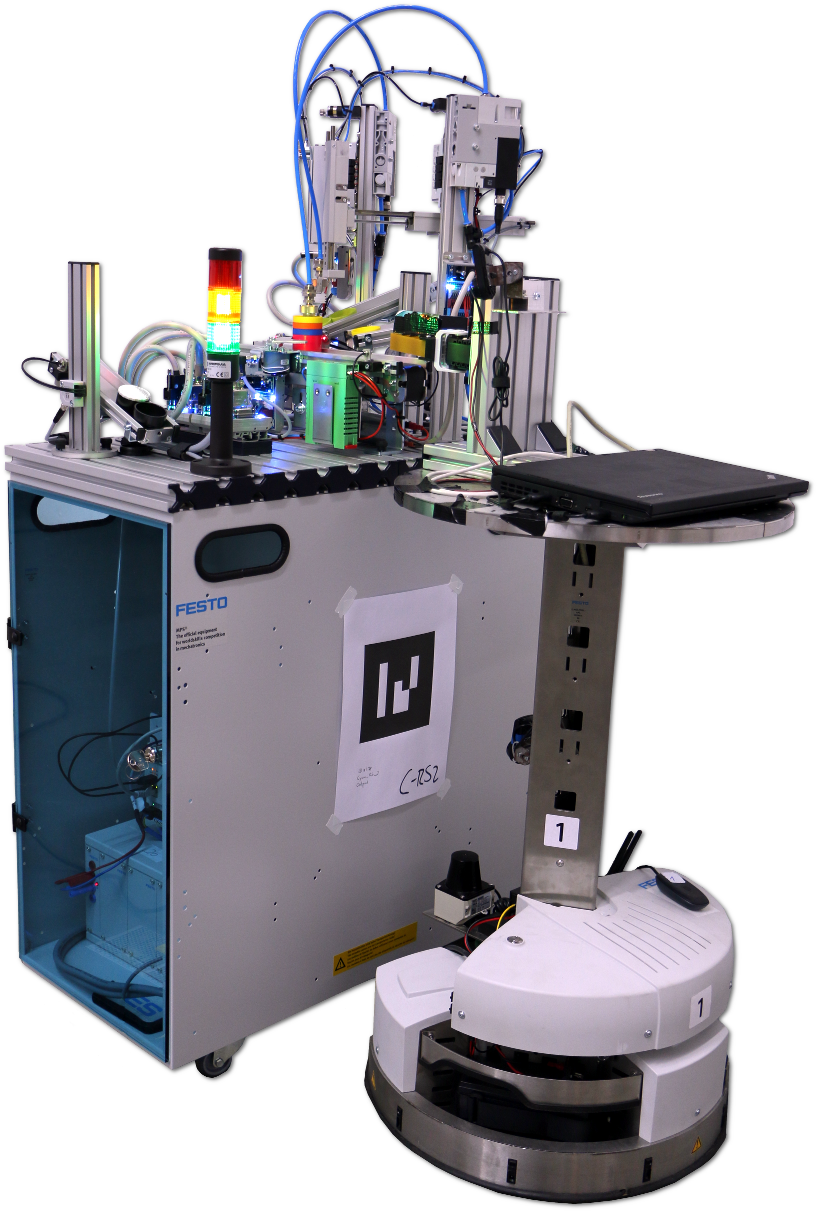
\includegraphics[width=0.3\textwidth]{img/rcll}
  \vspace{-4ex}
  \caption{Robot and MPS used in the RCLL}
  \label{fig:rcll}
\end{wrapfigure}

The \emph{RoboCup Logistics League (RCLL)}\footnote{RoboCup Logistics
  League website: \url{http://www.robocup-logistics.org}}
is a industry-oriented competition within RoboCup.  It tackles
the problem of production logistics in a smart factory where mobile
robots have to plan, execute, and optimize the material and production
flow between machines to produce and deliver products according to
dynamic orders. Competing teams deploy a group of up to three robots
which have to autonomously build ordered products by interacting with
\emph{Modular Production Machines (MPS)} and transporting workpieces
between these machines.  \reffig{fig:rcll} shows an RCLL robot filling
a machine which mounts colored rings on workpieces. The robots are
based on the Festo Robotino 3 platform which uses an holonomic drive,
and can be extended and programmed by the teams. The robot shown in
\reffig{fig:rcll} was build by the Carologistics team and used an
laser range finder for localization, a custom made gripper for
handling workpieces and several cameras for detection of AR-tags and
light-signals mounted on the machines~\cite{Carologistics2015}. The
game is controlled by a software component called \emph{referee box
  (refbox)} which randomizes the machine placement in the factory and
the production orders, communicates with the competing robots,
controls the machines and awards points.

The game consists of two phases~\cite{LLSF-Rules-2015}. In the first
phase, the \emph{exploration phase}, the robots have to roam the
factory to find randomly placed machines which are used later.
%% By detecting the light signal shown by the machines, the robots can
%% determine the machine-type. For correct reports of discovered machines
%% to the refbox the team is awarded points, for incorrect ones points
%% are subtracted.
%%
%% \begin{figure}[t]
%%   \centering
%%   \begin{minipage}{.8\linewidth}
%%   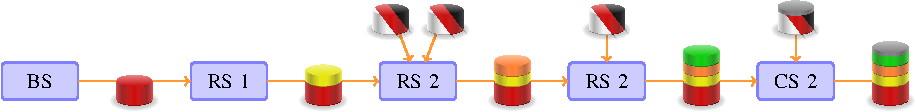
\includegraphics[width=\linewidth]{img/chain_c3}%
%%   \end{minipage}
%%   \quad%
%%   \begin{minipage}{.15\linewidth}
%%   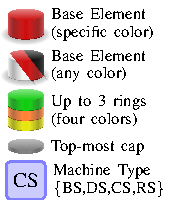
\includegraphics[width=\linewidth]{img/legend}%
%%   \end{minipage}
%%   \caption{Production chain of a high complexity
%%     product in the RCLL.}
%%   \vspace{-2mm}
%%   \label{fig:prod-chain}
%% \end{figure}
%
In the second phase, the \emph{produciton phase}, the refbox announces
orders, which products have to be produced by the robots. The products
are build from colored cups with optionally mounted rings and and a
colored cap.
%% \reffig{fig:prod-chain} shows the production chain to
%% build a high complexity product.
There are four different machine
types. The \emph{base-station (BS)} provides new bases, the colored
cups, as raw ressource. The \emph{ring stations (RS)} mounts colored
rings on a workpiece
%after preparing it with a varying amount ofbases.
The \emph{cap-station (CS)} mounts %black or grey
aps to finish a product
%after loading it with a cap form a shelf first.
The \emph{delivery-station (DS)} is used to deliver products.

The challenges of the RCLL lie in the dynamic and only partially
observable environment the robots have to robustly and fully
autonomously work in and in the planning and multi-robot coordination
required.
%% to build as many ordered products as possible and deliver
%% them in time given time window, and in the baseline robotic challenges
%% such as collision avoidance, perception and behavior execution. The
%% dynamism of the environment is caused by the ranomized factory layout,
%% randomized out-of-order times of machines, the highly customizable
%% amount of products that preclude producing in advance, unknown
%% obstacles, such as the other teams robots and hard to completely avoid
%% handling mistakes by the robots.
To cope with these challenges, a
multi-robot decision making is nesseccary and therefore a mechanism to
share knowledge about the world model between the robots. This can be
done by the robot memory which also allows combining a global planner
for finding almost optimal plans and a reasoner for plan execution.

\subsubsection{@Home League}
\begin{wrapfigure}{r}{0.3\textwidth}
  \centering
  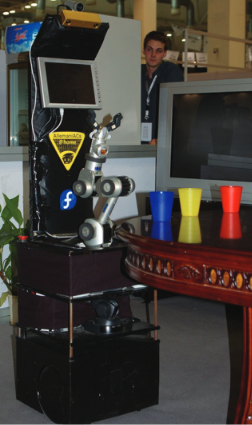
\includegraphics[height=150px]{img/ceasar}%
  \caption{RoboCup@Home robot tidying up~\cite{wisspeintner2009robocup}}
  \vspace{-2mm}
  \label{fig:athome}
\end{wrapfigure}

The RoboCup@Home league is a competition about domestic service
robots~\cite{wisspeintner2009robocup}. The robots have to assist
humans in a wide variety of everyday tasks. These tasks include
serving drinks, cleaning, setting tables, guiding or following people,
helping in emergency situations, shopping, cooking and
more. \reffig{fig:athome} shows an @Home robot in the
competition.
%
The goal of the RoboCup@Home league is to foster and benchmark
research in the area of domestic service robots, to build a research
community and to envision autonomous multi-purpose robots helping
humans and especially elder people in the personal life.

The competition consists of an open challenge and multiple subtasks
such as finding and manipulating objects, navigation tasks,
remembering persons, wait on tables and acting as
nurse~\cite{athome-rules}. To solve these challenges, robots need to
have a wide variaty of abilities, including navigation, object
detection and manipulation, speech recognition and especially human
robot interaction, which requires, for example, applying everyday
knowledge to incomplete task descriptions given by humans.

Important challenges in the @Home league are acting robustly in a
dynamic and only partial observable domestic environment where people
and objects can disappear or be moved without the robot recognizing
it. The robot memory can help here because it allows to collect a lot
of knowledge about the concrete domestic environment and, for example,
log object observations to learn their spatio-temporal distribution.
%% Furthermore, detecting and manipulating objects in a personal
%% environment can be difficult because the space the robot acts in, for
%% example the frige, can be very clouded.

\subsection{Fawkes Robot Software Framework}
\label{sec:fawkes}
The basis for the proposed thesis is the robot software framework
\emph{Fawkes}\footnote{\url{http://www.fawkesrobotics.org}}. It is
available as Open Source~\cite{FawkesDesign}.
%and developed at the Knowledge-based Systems
%Group\footnote{\url{http://www.kbsg.rwth-aachen.de}} (KBSG) at RWTH
%Aachen University
It is designed to work with a
plenthora of robots in different domains and follows a component-based
software design which separates functional entities into individual
software modules~\cite{component}. This enables reusing common
software solutions for robotic problems such as localization,
navigation, perception, reasoning and behavior execution. The binary
components can be loaded as \emph{plugins} at run-time.
%
Plugin activity is organized in threads to make use of multi-core
architectures. The threads can be run continously ore be hooked into
the main-loop of Fawkes to order the execution into a
\emph{sence-think-act} cycle to guararnee that higher-level components
can use the latest data. Furthermore, Fawkes guarantees loop times by
monitoring and eventually pausing and resuming threads running for too
long in one loop iteration.
% Ros blabla from BA?
Features in Fawkes are provided as \textit{aspects}. These aspects are
based on aspect-oriented programming~\cite{aspect_oriented} and give
access to a particular feature. Threads that want to use a feature can
inherit from the corresponding aspect. For example there are aspects
for accessing the blackboard, logging and timing~\cite{tnthesis}.

The communication between plugins is realized with a \emph{blackboard}
paradigm. The blackboard lists structured entries called
\emph{interfaces} which contain informaiton. Interfaces can be
provided by one plugin at a time, the writer, and read by other
plugins, the readers. This allows a very flexible communication
because the information provision in the interface is decoupled from
the concrete components which use the information and plugins writing
to the interfaces can be exchanged, e.g. by simulation plugins writing
to the same interface. Furthermore, the blackboard architecture
simplifies debugging because the current communication between two
plugins, determined by the state of the interface, can be viewed and
logged at runtime. To send commands to an interface writer, e.g. a
motor command to the motor controller, readers can send messages to
the interface.

As a communication infrastructure between different components, the
blackboard is one possibility to realize a robot memory shared between
multiple planners and reasoners in the current version of
Fawkes. Indeed the blackboard works well for providing information and
sending commands, though there are major limitations for this
application. One limitation is the strict rule, that only one
component can write an interface to provide information. This rule is
very usefull to avoid problems in standart plugin communication but
obstructive for multiple components sharing common information. For
example when a reasoner concludes that a product is placed at the
machine output after the production time and a behavior execution
component concludes that the robot holds the product after the grabing
action succeded, both components would have to modify the same piece
of information in the shared robot memory. Another limitation is the
fixed size and structure of blackboard interfaces. Therefore it is not
possible to dynamically represent more information, such as positions
of detected objects, than initially defined. Furthermore, the blackboard
does not support long-time memory.

\subsection{Planners and Reasoners}
\label{sec:planners}
This subsection gives an overview of planners and reasoners which are
going to profit from using and communicating with the robot
memory. For the variety of these, we give four
examples which should use the robot memory to achieve new or improved
functionality and to evaluate this thesis. The example planner and
reasoner systems are \emph{CLIPS}, a rule-based production system,
\emph{Golog}, a high-level programming language based on the Situation
Calculus, and the \emph{Planning Domain Definition Language (PDDL)},
which incorporates a family of planning formalisms into a standart
programming language. These examples are representatives for often
used types of planners and reasoners. However, the robot memory should
not be limited to these examples and provide a general C++ interface.

\subsubsection{CLIPS rules engine} The reasoner we currently use in the RCLL
to implement the high-level game agent is the rule-based production
system CLIPS which uses forward chaining based on the Rete
algorithm~\cite{Rete}. CLIPS consists of a fact-base, which is a
working memory with many small pieces of information, a knowledge base
with rules and procedures, and an inference engine~\cite{CLIPS-RM}
working with the knowledge base on the fact-base. The pieces of
information in the fact-base are called facts and consist of a name
and a key-value structure defined in a template for \emph{unordered
  facts}
(e.g. \textit{(position~(name~robot1)~(translation~2.5~1.0~0.0)}) or
an ordered list of values for \emph{ordered facts}.
\begin{figure}
\begin{lstlisting}[showlines,style=ReallySmallCLIPS, caption={CLIPS
    rule to change a robots state when the object it searched for is visible.},
  label=lst:clips-rule,
  emph={skill, args, state, target, res},
  emphstyle=\bfseries\color{green!80!black},
  emph={[2]\?skill, \$\?args, wait-for-lock, \?target, use,
  WAIT-FOR-LOCK, SKILL-EXECUTION, running},
  emphstyle={[2]\bfseries\color{blue!80!black}},
  morekeywords={retract, assert, modify, skill-call, skill-to-execute,
  wait-for-lock}]
(defrule found-machine
  ?s <- (state SEARCHING_FOR ?machine)
  (visible  (name ?machine))
  (position (name robot1) (translation $?pos))
  =>  
  (retract ?s) 
  (assert (state IDLE))
  (printout t "Found machine " ?machine " at " ?pos crlf)
)
\end{lstlisting} %$ This is just to fix Emacs highlighting due to dollar sign in code above
\end{figure}
An example rule is shown in \reflst{lst:clips-rule}. Rules are
composed of an \emph{antecedent} and a \emph{consequent}. The
antecendent is written before $=>$ and describes the contition that
has to be satisfied before the the rule is activated. It consists of a
list of patterns that have to be matched by the fact-base. For the
antecendent in \reflst{lst:clips-rule} there have to be fitting
\textit{state}, \textit{visible}, and \textit{position} facts where
$?$ and $\$?$ mark variables. The consequent is the part behind $=>$
and defines the procedure that is executed when the rule is
activated. It usually modifies the fact-base by retracting and
asserting facts as in the example to remove the old and add a new
state fact. The inference engine is responsible for checking which
rule antecendents are satisfied by the fact-base. If multiple rules
could fire, the inference engine chooses the rule with the highest
priority, executes the consequent and checks again. \emph{Functions}
can be called in the consequent, can have side effects and also be
implemented in C++. The RCLL agent implemented in CLIPS represents its
knowledge about the state of the world, the \emph{world model}, in its
fact-base. It controls which actions are taken by the robot by using a
technique called \emph{Incremental Reasoning}~\cite{CLIPS-Agent}. This
basically means that, whenever the robot is idle, it searches for the
next best task and executes it. For each task there is a rule with its
preconditions in the antecendent and the actions to take in the
consequent. There are also rules for modifying the worldmodel
(e.g. after finishing actions or getting new sensor data), task
execution, coordination with other robots and more. The coordination
of the robot team includes synchronizing their world model, so each
robot knows what other robots noticed and changed in the environment,
and resource allocation to ensure no two robots try to use the same
machine at a time or try to achieve the same goal by choosing a
redundant task. This coordination is currently implemented in CLIPS
rules using Profobuf\footnote{Google Protocol Buffers}
messages. Alternatively, this could also be done by using a
distributed robot memory which contains the world model in a
distributed database. This would be advantageous
because the database already provides efficient synchronization and
the implementation in CLIPS is not convinient due to its
specialization on logical rules.


\subsubsection{Planning Domain Definition Language (PDDL)} PDDL is a
standardized language for planning problems~\cite{PDDL}. It allows
modeling the nature and behavior of a domain as well as the
\emph{actions} possible to perform in a \emph{problem
  description}. With an additional \emph{problem description} which
defines the problem to solve it can be given to a PDDL planner which
searches for a totally or partially ordered sequence of actions, the
\emph{plan}, to solve the problem.
%% \todo{action example}
%% \reflst{lsf:pddl-action} shows an example action contained in a domain
%% description.
Actions consist of preconditions and effects.  There are
various versions and extensions of PDDL which introduce new concepts
and features. A version often used in RoboCup domains is
PDDL~2.1~\cite{PDDL2.1} \todo{really?}. It adds numeric values and
continous actions. This allows finding optimal plans in continous
environments where, for example, distances and travel times
matter. PDDl has the advantage of being able to find comlete and
optimal, or at least efficient, plans. However, this comes with the
drawbacks of high computational effort for larger domains and the
problem of adopting to events during plan execution. For example when
the domain is not fully observable, the robot could sense changes in
the environment or fail executing an action. This would require
notifying the planner, incorporating the changes in PDDL and
replanning. To solve this problem we want to combine PDDL with an
execution in CLIPS. Then PDDL generates an efficient and complete plan
with coarse actions and CLIPS executes the plan action for action,
while monitoring the execution and updating the worldmodel according
to percieved changes. This world model is written into the robot
memory so that PDDL can access the world model with all applied
changes. This way the strenghtes of both PDDL and CLIPS.


\subsubsection{Golog } Golog is a high-level programming language based on the
\emph{Situation Calculus}, a first order logic formalism for knowledge
representation and reasoning in dynamic domains~\cite{Golog}. It
allows representing world states as terms called
\emph{situations}. These can be used in relations and functions called
\emph{fluents}. (e.g. $holding(x,s)$ is a fluent representing if
object $x$ is hold by the robot in situation $s$.) \emph{Actions} can
lead to new situations (e.g. $s'=do(pickup(x),s)$) and are modeled
with \emph{precondition axioms} (e.g. $Poss(pickup(x),s) \equiv
\forall y [\neg holding(y,s)]$). The value of relational fluents after
performing actions is defined by \emph{successor state axioms}
(e.g. $Poss(drop(x),s) \supset [broken(x,do(a,s)) \equiv a=drop(x)
  \wedge fragile(x) \vee broken(x,s) \wedge \neg a=repair(x)]$).
Golog as a high-level programming laguage features imperative
programming constructs such as procedures, conditions and loops as
well as nondeterministic branching. There are multiple dialects of
Golog which add features needed for robotic
applications. ConGolog~\cite{ConGolog} adds concurrency and
interrupts, IndiGolog~\cite{IndiGolog} adds on-line execution of
programs and sensing actions, which determine the value of a fluent
during execution, and ReadyLog~\cite{ferrein08ras} extends IndiGolog
with passive sensing during the execution of other actions. With these
dialects, Golog has been proven as useful for robot applications in
multiple domains such as domestic service robots. By providing an
interface to the robot memory, the strengthes of Golog, the highly
expressive behavior specification, can be combined with other
approaches to compensate the weaknesses, e.g. unefficient
planning~\cite{Golog-Planning}. There already are approaches to
combine Golog an PDDL into a continous planning framework that uses
PDDL for planning and Golog for execution and expanding placeholder
actions into sub-plans based on current information unavailable during
initial planning~\cite{ContPlanGolog}. It is implemented with a
translation between PDDL and
Golog~\cite{Golog-PDDL-Trans}. Furthermore, the robot memory could be
useful as additional persistent and distributed knowledge storage
(e.g. for saving the context during an interrupt
\todo{cite Gesche Interrupts}
and resuming the task by another robot).

\subsubsection{Motion Planners:}
Another kind of widely used planner in robotics are motion
planners. They usually plan the motion of a robotic arm to reach a
certain goal position where an object should be grabed or placed. A
motion planner needs to find a trajectory from the initial position to
the goal position, taking joints of the arm into account and avoiding
collisions with objects in the environment. A widely used motion
planner is MoveIt which is available for ROS and the PR2
robot~\cite{MoveIt}. Another motion planner already integrated into
Fawkes is OpenRave~\cite{OpenRave}. These planners could benefit from
using a robot memory by accessing and sharing information about
objects and obstacles in the environment and by informing other
planners and task execution components about the outcome of a motion
plan (e.g. about the cause that prohibited the motion). This
especially requires the robot memory to represent hybrid knowledge in
the form of continous positions and time related events.

\subsection{MongoDB}
\label{sec:mongodb}

%% Since storing, keeping and retrieving knowledge of the robot memory
%% are central tasks of this thesis, the choise of a database
%% implementation is important.
MongoDB is a \emph{document-oriented}
database which fits particularly well for application in this thesis. It
provides many useful features which would take a large effort to
implement manually, has proven as powerful and scalable data
storage~\cite{mongodb,RoboDB} and is widely used. In contrast to
relational databases, document-oriented ones store entities called
\emph{documents} consisting of key-value pairs.
\begin{figure}
  \begin{minipage}{0.6\linewidth}
\begin{lstlisting}[style=SmallJSON,
  caption={MongoDB document representing\\ the position of a robot},
  label=lst:mongo-document,
  framexleftmargin=2pt, xleftmargin=2pt,
 morekeywords={}, numbers=none]
 {
   _id: ObjectId("573e7cfbb2af949d9"),
   type: "position",
   name: "robot1",
   translation: {x:2.5, y:1.0, z:0.0},
   rotation: {x:0.0, y:0.0, z:0.0, w:1.0},
   timestamp : ISODate("2016-05-19T15:26:34.466Z")
 }
\end{lstlisting}
  \end{minipage}
  \begin{minipage}{0.4\linewidth}
\begin{lstlisting}[style=SmallJSON,
  caption={MongoDB query for the document in \reflst{lst:mongo-document}},
  label=lst:mongo-query,
  framexleftmargin=2pt, xleftmargin=10pt,
 morekeywords={}, numbers=none]
db.positions.find(
  {
    type: "position",
    name: "robot1",
    timestamp : {"$gt": ISODate(
      "2016-05-19T15:26:34.000Z")}
  })
\end{lstlisting}
  \end{minipage}
\end{figure}
\reflst{lst:mongo-document} shows such a document
%used for storing the position of a robot.
The different
values can be accessed by their key and can have different types, such
as strings, numbers, complexer objects (e.g. dates) and nested
sub-documents (e.g. translation containing 3D coordinates). In
contrast to relational databases, there is no predefined schema that
enforces the structure of documents. However, documents with similar
structure are usually grouped into \emph{collections}. Therefore the
documents inserted in a collection implicitly define the structure
during runtime. This allows a flexible use of the database because
applications are not limited to a fixed schema and can, for example,
add key-value pairs during runtime when additional information needs
to be stored.
%% Furthermore, this simlyfies development in which the
%% document structure tends to change often. Even if there are documents
%% with different structure, the application can choose to retrieve only
%% certain documents by giving a specialized query.
Queries in MongoDB are similar to documents because the arguments of
query funcitons also use document structure. An example query is
shown in \reflst{lst:mongo-query}. It searches for all documents in
the collection \texttt{positions}
%of the current database
that have matching  values for \texttt{type} and \texttt{position} and
are up to date, thus with a timestamp greater than the given
one. Multiple key-value pairs in a query are conjunctive.
Values can be checked and compared as in the example
with a variety of operators such as \textit{not}, \textit{or},
\textit{and}, \textit{equals}, and \textit{greater than}. These
queries can be evaluated very quickly, especially when \emph{Indexing}
is used, a database feature that manages indexes for a combination of
document keys.
%todo continue shortening
For more complex queries it is
possible to add arbitrary JavaScript functions with the \textit{where}
operator to check if documents match the query. Furthermore, it is
possible to aggregate results using the \emph{Map-Reduce} paradigm
which maps resulting documents to intermediate documents which are
then reduced until the end-result is found. For example this allows
querying for the nearest visible object by getting all visible
objects, mapping their position to a distance and reducing them to the
nearest one by dropping more distant ones when comparing them.  The
higher expressiveness of these queries comes with the price of slower
computation. However, the computational effort can be reduced by
formulating queries smartly. Many usual queries,
e.g. \reflst{lst:mongo-query}, can be formulated without using
\textit{where} operators. Furthermore, complex queries can be nested
to filter documents first with a fast query and execute the
computationally costly query only on the remaining documents.
%
An especially useful feature of MongoDB which allows sharing knowledge
between multiple robots is \emph{replication}. Replication is a
process that distributes a database onto multiple machines.
One MongoDB instance called \emph{Master} initially
copies the database  to other instances called \emph{Slaves}.
Afterwards, all modifications to the master database, which are
stored in a separate collection called \emph{Oplog}, are forwarded to
the slave to keep them synchronized and consistent.
%% This is often used
%% in web-services to distribute read-queries and their computation on
%% multiple machines and to keep backups.
Read only queries can be
computed by Master and Slave instances, modifying queries are
forwarded to the Master to garantee consistency.
MongoDB can also group multiple
instances into a \emph{Replica Sets} which automatically manages
the master election when necessary. Using replication,
multiple robots can robustly share a common and consistent world
model. Robot specific knowledge can be kept in a seperate and not
replicated collection to avoid unneded communication.
%% There also exist
%% extensions of MongoDB which implement a \emph{Multi-Master
%%   Replication}. This would enable writing to each instance immediately
%% and synchronizing the changes later. \todo{source} This allows faster
%% writing especially if the Master is not available for some time but
%% requires to resolve write conflicts and handle them in the
%% application. Thus Master-Slave Replication is more convinient for the
%% applicaiton.
%% There are also extensions of MongoDB providing so called \emph{Trigers} which
%% can notify an application if something in the database changes as
%% previouly defined. \todo{source} These Triggers use the Oplog of
%% MongoDB to find changes and are useful for planners. For example if a
%% global planner determined a plan that is being executed and wants to
%% be notified, if a condition changes that makes the plan invalid, to
%% replan.

MongoDB is especially well suited for this thesis because of its
performance and scalability compared to other document-oriented
databases with similar features. A possible alternative to MongoDB is
the document-oriented database CouchDB~\cite{CouchDB}. CouchDB
focuses more on distributed Systems providing a system called
Multi-Master Replication which allows writing to all replication instances.
Conflicts can be solved similar to a version
control system, thus multiple conflicting versions can be kept in
parallel for later revision. However, MongoDB has shown to scale much
better than CouchDB and other document-oriented databases~\cite{db-comparison}.

%% \begin{itemize}
%% \item BSON JSON format for documents
%% \item JavaScript example
%% \item Capped collections?
%% \item dreieck comparison ?
%% \item GridFS file storage?
%% \end{itemize}

\section{Related Work}
\label{sec:related}
\subsection{KnowRob}
\label{sec:knowrob}
KnowRob is an open source knowledge processing system for
cognition-enabled robots~\cite{KnowRob,KnowRob-Representation}. It is
designed to store knowledge about the environment and set it into
relation to common sense knowledge to understand vaguely described
tasks such as "set the table". For storage and inference of knowledge,
KnowRob uses Description Logic and approaches of the semantic web, an
effort to make websites machine understandable, and the logic
programming language Prolog for implementation. Each small piece of
information is represented as a \emph{Resource Description Framework
  (RDF) triple} (e.g. $rdf(robot, holding, cup)$) which are composed
of a subject, predicate and object. Commonsense knowledge is
represented in the \emph{Web Ontology Language (OWL)}. It uses
\emph{ontologies} which can roughly be described as directed graphs
setting objects or classes of objects into relation. The graph can be
represented with multiple RDF triples, where the subject and object
are nodes and the predicate is a directed edge from the subject to the
object. In these ontologies it is possible to represent common sense
knowledge such as "milk is-a perishable", "refrigerator
storage-place-for perishable", and "refrigerator is-a
box-container". Thus a robot asked to bring milk could infere that the
milk is stored in the refrigerator which needs to be opened first
since it is a box-like container.  To be able to interface the
perception of a robotic system, KnowRob uses a concept called
\emph{virtual knowledge base}. It allows computing needed information
on demand instead of storing everything providently. Thus special
queries can be forwarded to other components which compute the answer
efficiently. Especially for perception based on sensor data or
transformation of spational relations, this is advantageous compared
to continously computing the results for all possible queries and
storing them. The concept inspired the usage of virtual knowledge
bases in this thesis. KnowRob implements it with Prolog predicates
called \emph{Computables} which call C++ functions of other
components. This indeed slows down the computation of a query but is
more efficient than continously computing and storing the results or
implementing and computing the other components algorithms in Prolog.
To understand the robots environment large and detailed ontologies are
necessary. KnowRob features aquireing and connecting these from
various sources such as online common sense databases, the cloud-based
robot infrastructure RoboEarth and websites made for humans for
deriving object information from internet shops and action recipies
from howto websites. However, it has been found that this aquired
knowledge needs a lot of manual extension and verification before it
can be used~\cite{KnowRob-Web}. Encyclopedial knowledge often lacks
action information needed by the robot (e.g. how to grab tools) and
action recepies require human text understanding. Furthermore large
ontologies limit the performance of KnowRob because of the Prolog
implementation and general complexity. Although KnowRob features
usefull concepts such as common sense reasoning with ontologies and
virtual knowledge bases we do not use it as a basis for a robot memory
in Fawkes because of missing support knowledge shared between multiple
robots and a too strong focus on data only for reasoning components or
respectively performance and scalability concerns with Prolog handling
larger datasets (e.g. storing locations of found object over long time
to learn the distribution where they can be found).

\subsection{OpenRobots Ontology (ORO)}
\label{sec:oro}
The OpenRobots Ontology (ORO) is an open source knowledge processing
framework for robotics~\cite{Oro}. It features commonsense ontologies
similar to KnowRob and is designed to enable human-robot
interaction. It also uses RDF triples and OWL ontologies. The triple
storage is implemented in Jena, a Java toolkit for RDF, and the
inference with Pellet, a Java OWL reasoner. Besides knowledge storing,
querying and reasoning, ORO features a modular architecture between
the back-end storage and front end socket server for querying. These
modules add features such as events that notify external components
about changes (e.g. if instances of certain classes are added or
modyfied). Another module adds representations of alternative
perspectives that should allow understanding difficult situations with
multiple agents. For example when a human asks a robot to bring the
cup, there are two cups on a table and the robot should infer which
cup is meant by knowing that the other cup is occluded from the humans
point of view. Furthermore ORO features categorization to find
differences between objects (e.g. to ask if the blue cup or the red
cup was meant in a vague task description) and Memory profiles for
distinguishing long-term knowledge and short-term knowledge which is
removed when the lifetime of a fact exires. Although these are usefull
features and we want to realize the concepts of events and memory
profiles in this thesis, we do not use ORO as a basis. Due to its
focus on human-robot interaction and commonsense reasoning, it is not
suitable for representing large amounts of data for non reasoning
components because all data would have to be stored in RDF tripels and
processed by the OWL reasoner. Furthermore, it does neither support
synchronizing a part of the knowledge with other robots nor a virtual
knowledge base.

\subsection{Generic Robot Database with MongoDB}
\label{sec:mongo-logging}
There already is a generic robot database developed with MongoDB as
data storage~\cite{RoboDB}. It is primarily used to log data of a
robot middleware (Fawkes and ROS) for fault analysis and performance
evaluation. To achieve this, it taps into the messaging infrastructure
in ROS and the blackboard interfaces in Fawkes to store the data one
to one utilizing the flexibility of the schema free MongoDB. The
logged data can later be queried by the robot or a developer. This
allows better evaluation and fault analysis because the data would
otherwise be disposed and logging of the whole
Data-Information-Knowledge-Wisdom (DIKW) hierarchy~\cite{DIKW} enables
retracing processes such as from point clouds (data) to cluster
positions (information) to object positions (data) combined from
multiple clues to learning results (wisdom). This work already
implemented a basic connection to MongoDB in Fawkes for storing
documents and executing queries, which can be used in this thesis. It
also showed that MongoDB is a good choise because it can handle
querying a large dabase and writing a lot of data efficiently while
being flexible how an which kind of data is being represented.
However this work lacks some important concepts needed for a robot
memory as intended in this thesis. It is intended as logging facility
and not as working memory holding a world model for multiple planners
and reasoners. Therefore updating and querying mechanisms for planners
and reasoners are missing as well as triggers, a virtual knowledge
base and multi-robot synchronization.

\subsection{Open-EASE}
\label{sec:openease}
Open-EASE is a knowledge processing service for robots and AI
researchers~\cite{OpenEASE}. It is based on and combines
KnowRob~\cite{KnowRob} and the Generic Robot Database with MongoDB in
ROS~\cite{RoboDB}. It is designed as a web service accessible by
robots via a socket connection and by humans via a web browser. It
uses KnowRob for commonsense reasoning and storing the world model of
a robot. The Generic Robot Database is used to log data about robots
or humans performing manipulation tasks. This data can then be
accessed by using computables of the virtual knowledge base concept to
learn from human demonstration and analyze and learn from faults. The
focus of Open-EASE also is on providing the recorded data and access
to KnowRob to humans using the web interface. This allows using
Open-EASE as eLearning tool for students, who can explore and
experiment with the data and system on the robot. Furthermore it
fosters reproducing experiment results (e.g. for reviews) and
visualizing them. Although the system is accessible from multiple
users and robots which can query the same Open-EASE instance, it is
focused on single robot data and non collaborative processes because
each user operates in his private container with individual knowledge
base. This makes sense in the context of student exercizes. If the
system is also usable or being extended for cooperating robots or
planners exchanging knowledge over the web service is not mentioned in
current publications or on the project
website\footnote{\url{http://www.open-ease.org/}}.


\section{Approach}
\label{sec:approach}
This section presents the approach of the proposed thesis. It starts
with the goals we want to achieve with the robot memory and why they
are useful for the application. It follows an overview of the
architecture which describes in which components the robot memory is
organized and how they interact with each other. Afterwards, we
describe how the implementation is planned, especially for the robot
memory and the interface using planners, reasoners and other
components. We finish the presentation of the apprach with a section
how to evaluate the robot memory qualitatively and quantitatively and
give a time schedule for the thesis.

\subsection{Goals}
\label{sec:goals}

This subsection presents the goals of this thesis and why we want to
achieve them:

\smallskip
\textbf{Flexible Storage and Retrieval:} The robot memory has to
provide a service for storing, updating, removing and querying so that
different components can use the robot memory to provide knowledge,
use it as a source, or collaborate using the same memory. It should be
flexible enough to store any kind of data, information, knowledge, and
wisdom of the DIKW hierarchy in any structure. For example the robot
memory should be able to store a world model, perception results and
even large datasets such as remermbered sights of objects for later
learning and user preferences.

\smallskip
\textbf{Collaboration of Planners, Reasoners and Other Components:}
The robot memory has to allow multiple components to collaborate by
sharing a common database. This should especially be used to share a
common world model between different kinds of planners and reasoners
to combine their special strenghts and componensate their
weaknesses. For example PDDL can generate global and optimal plans
which are executed and monitored by CLIPS that can react better to
different situations during execution. Through using the robot memory,
both can share a common world model so that changes found and applied
to the world model by CLIPS are directly available in PDDL (e.g. in
case replanning is necessary because the previous plan is not feasable
anymore).

\smallskip
\textbf{Special Views for Different Components:} Depending on the
application of different components using the robot memory, different
views on the stored data is necessary. For example a planning
components needs another part of the stored data, than a component
learning distributions of object sights. Thus component specific
filters are necessary. Furthermore, different components need the
stored data in different formats (e.g. depending on the used
programming language). Keys or identifyers might be named differently
and have to be translated.

\smallskip
\textbf{Virtual Knowledge Base:} The robot memory has to prodive
access to virtual knowledge. This is knowledge which is not stored in
the robot memory directly, but computed on demand. This allows
accessing knowledge through the robot memory that is otherwise
impractable to compute and store continously and for all possible
queries. For example when a component queries the distance of two
objects, it is better to compute the result on demand taking both
concrete objects into account than to store all distances between each
two objects in the memory and to update these values continously.
When components using the robot memory can also provide computation
functions for virtual knowledge to the robot memor, this adds a lot of
versitality and expandability. For exapmle it would be possible to add
a commonsense reasoner similar to KnowRob or ORO providing virtual
knowledge to the robot memory. Queries for this commonsense knowledge
would then be forwarded to the commonsense reasoner and be solved by
relating knowledge in the memory to an ontology.

\smallskip
\textbf{Shared Knowledge for Multi-Robot Systems:} The robot memory
should be able to distribute parts of the knowledge over multiple
robots which can then share a common world model necessary for
collaboration. The concept is similar to multiple planners sharing a
world model with the differnence that the components on a multi-robot
system work simultaniously and the additional difficulty to
synchronize the robot memory between the robots. Such a distributed
robot-memory is necessary in many multi-robot domains, especially the
RCLL where the whole robot team needs to know the world model
(e.g. where other robots placed intermediate products) and what other
robots intend to achieve at the moment. If the distribution of the
knowledge would not be implemented in the robot memory it would have
to be implemented seperately. Distributing the robot memory adds
additional requirements and challenges, especially robustness (e.g. in
the case of robots dropping out), consistency of the memory, and
accessibility so each robot can use the robot memory without large
latencies.

\smallskip
\textbf{Spatio-Temporal Grounding:} It is often desirable to ground
stored knowledge based on location and time because this allows many
applications such as spatio-temporal clustering, using old
observations to deal with the assignment problem, and learn
distributions (e.g. at which daytimes objects can be found at which
positions). Thus the robot memory has to be able to store knowledge
tagged with spatio-temporal information and consider this information
while querying.

\smallskip
\textbf{Event Triggers:} The robot memory should be able to notify
components about changes in the memory which are relevant for
them. These notifications are called \emph{event triggers} and should
automatically be sent after a component registers an event it wants to
be notified about. These events include appearences of new instances
of a specific knowledge type, modifications and deletions of it as
well as sentences becoming true or queries returning documents. The
balance of expressiveness versus performance still needs to be
found. A use case in which event triggers are especially useful are
when planners want to be notified when their plan becomomes unfeasable
and replanning is necessary. In this case, the planner could for
example register events for the plan execution being aborted or
preconditions of a plan becoming false.

\smallskip
\textbf{Modular Extentions:} The robot memory should be expandable
with various modules imlementing additional functionality. An
interesting example module could introduce knowledge decay for
removing knowledge with exceeded lifetimes. This would allow
differentiating short-term knowledge and long-term knowledge. Other
modules could, for example, add confidence values or abstraction
levels to stored knowledge. Furthermore, extensions such as robot
memory initialization from a saved file, saving parts of the memory to
a file and a logging facility similar to the generic robot database
would be useful.


\smallskip
\textbf{Persistent Storage:} To profit from long-time knowledge and to
operate robots over long time as neccessary in the intended domains
such as domestic service, the knowledge needs to be stored
persistently. This way, it is not lost when restarting a robot or
repeating an experiment depending on knowledge stored in the robot
memory.

\smallskip
\textbf{Human Interface and Visualization:} An important factor in the
development of a robotic systems is the accessibility of underlying
components for easier debugging and modeling. Therefore the robot
memory needs to provide an interface for developers to monitor the
state of the robot memory and to modify it. A visualization would also
be desierable to analyze spatio-temporal data efficiently.


\subsection{Architecture}
\label{sec:arch}
This subsection presents the architecture of the robot memory and
explains its design consideration. It shows how the intended
functionality is organized in smaller components and how these
components interact with each other.  The architecture in general
contains standart concepts of software
engeneering~\cite{software-architecture} and design pattern
considerations~\cite{design-patterns} to allow reusability and
adaptability to changing requirements and use cases. The most
important concepts are a layered architecture, functional abstraction
(e.g. of the different processes happening during storing and
querying), and data abstraction (e.g. of stored knowledge which is
more specialized internally than visible from a using
application). \reffig{fig:arch} shows the architecture of the robot
memory and is explained in the following.
\todo[inline]{move arch-figure so it is easily viewable when reading}
\begin{figure}
  \centering
  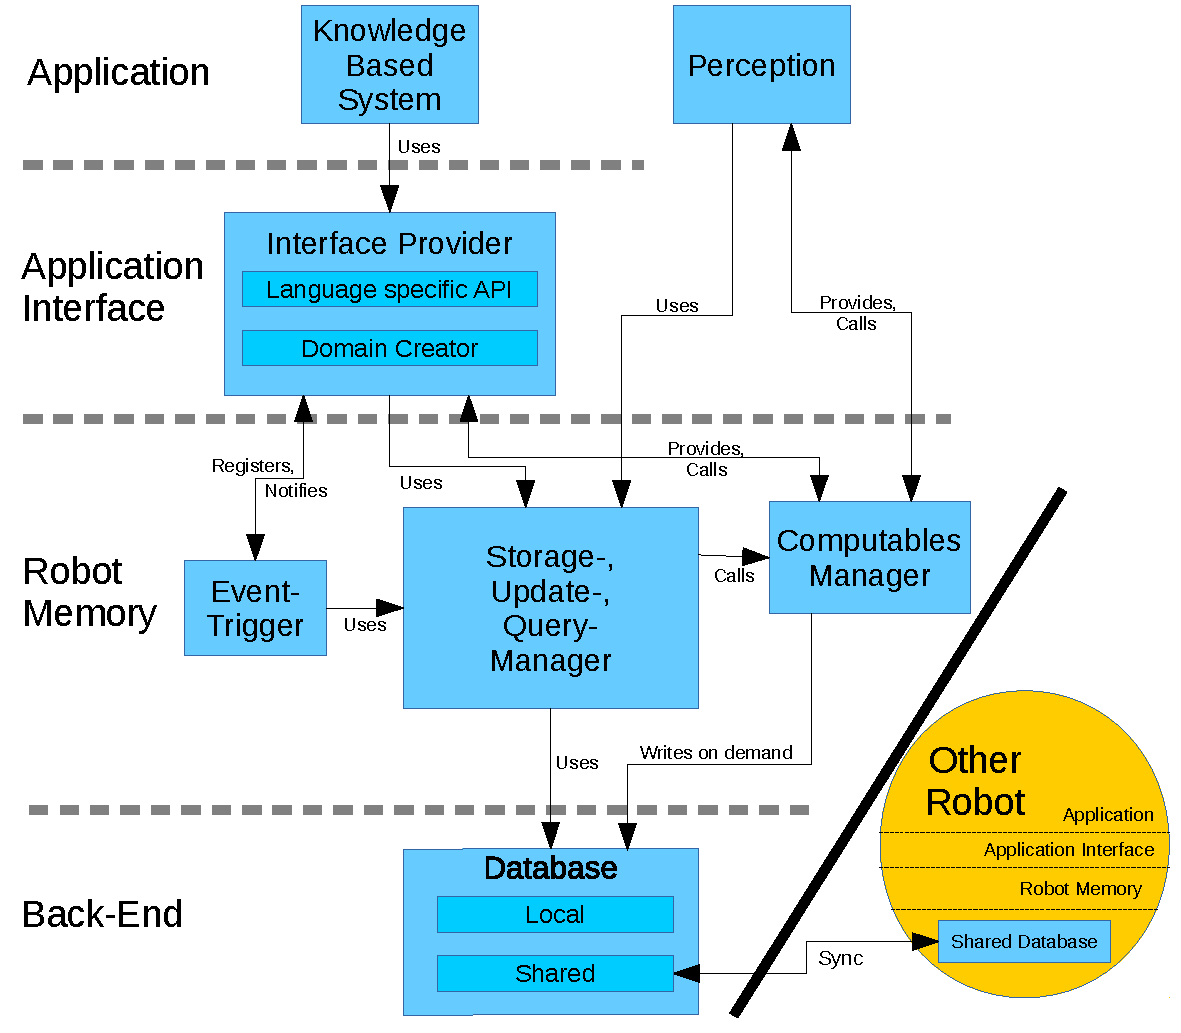
\includegraphics[width=0.9\textwidth]{architecture.pdf}
  \caption{Software architecture of the Robot Memory}
  \label{fig:arch}
\end{figure}
The architecture organizes all components relevant for the robot
memory into four layers: Back-End, Robot Memory, Application Interface
and Application. The Back-End contains the MongoDB databases where the
knowledge is stored and queries are executed. There is a private
database and a shared database distributed between multiple robots
using the same architecture. This distribution utilizes the efficient
replication features of MongoDB and avoids additional overhead. The
Robot Memory-layer contains the central functions that distinguish the
robot memory from a pure MongoDB database. It contains the Storage-,
Update- and Querymanager which is an intermediate component that
realizes most of the robot memorys functionality by modifying and
enhancing queries, storage and update requests before applying them to
MongoDB. If a query asks for virtual knowledge, the manager forwards
the query to the virtual knowledge base. The virtual knowledge base
manages which virtual knowledge is provided by which application and
requests the computation of virtual knowledge when demanded. The
component responsible for event-triggers receives and manages
registrations of applications that want to be notified in the case of
an event, uses the Querymanager to check if events happen and notifies
applications accordingly. Additional modules can be added to extend
the functionality of the Storage-, Update- and Querymanager. These
extensions use the ---Compositor
Pattern~\cite{design-patterns}\todo{check name} --- and therefore work
compositionally and dynamically. Between the robot memory and a
planner (or reasoner) component is the Application Interface layer. It
includes the Interface Provider component which makes the function of
the robot memory, which are accessable in C++, available to the
planner and the special programming language used by the planner. It
is not necessary for components that can directly use the C++
interface of the robot memory. The central task of wrapping the robot
memory functions into the planner programming language also includes
bringing query results in the appropriate format used by the planner
and eventually renaming key-names when they have be mapped to match
the names used in the planner domain model. Because planning and
reasoning languages and concepts can be very different, each planner
and reasoner needs a separate Interface Provider. The Interface
Provider can also contain a domain creator which creates the planning
domain and problem definition from a template and additional knowledge
from query results. For example, this is useful for PDDL planners
which would automatically get problem definitions updated to the
current world model stored in the robot memory. Finaly the Application
layer contains all components using the robot memory eigther through
the Interface provider or directly through the C++
interface. Application components can also register event-triggers and
provide computation functions for the virtual knowledge base.  The
knowledge aquisition filling the robot memory is devided between the
applications using the robot memory. Additionally, the Initializer
module can provide the initial knowledge from a file (e.g. for the
world model of a new RCLL game).


\subsection{Implementation}
\label{sec:impl}
This subsection covers the considerations for the impementation. It is
separated according to the layered architecture. Both application
layers are represented by the planner and reasoner part, because all
other application components (e.g. for perception) can simply use the
C++ interface of the robot memory.

\subsubsection{Back-End}
\label{sec:back-end}
The back-end is realized with MongoDB, acts as storage of the robot
memory and executes queries. The representation of stored knowledge
utilizes the document structure of MongoDB with key-value pairs and
nested subdocuments. This allows a very flexible storage of
knowledge-pieces with any additional properties needed by the
application. An example document stored in the back-end is shown in
\reflst{lst:backend}. 
\begin{figure}
\begin{lstlisting}[style=SmallJSON,
  caption={Representation of a knowledge piece in the back-end},
  label=lst:backend,
  framexleftmargin=15pt, xleftmargin=15pt,
 morekeywords={}]
 {
   _id: ObjectId("983e7cfbb2af16b5443949h5"),
   robot_memory_info:
   {
     persistent: true,
     decay_time: ISODate("2016-05-19T23:50:00.000Z")
   },
   type: "object info",
   name: "milk_1",
   position: {x: 2.5, y: 1.0, z: 0.0},
   storage_place: "refrigerator",
   fat_percentage: 3.5
 }
\end{lstlisting}
\end{figure}
It contains knowledge about a bottle of milk as it could be needed by
a planner with additional information where it should be stored
later. Additionally the document contains meta information needed by
the robot memory (e.g. if the document should be stored persistently
or removed at restart and when it should be dropped because it is
usetime has expired). The MongoDB back-end also manages the
distribution of knowledge between multiple robots. A part of the robot
memory is only locally relevant. The other part that should be shared
has to be set up as MongoDB replica set as already described in
\refsec{sec:mongodb}. This ensures that no unnecessary data is sent
over the network. The other proplems of a distributed database such as
consistency, master election and synchronization are solved by
MongoDB. The back-end also contains the Oplog of MongoDB, a separate
capped collection containing a list of all changes to the database
with a timestamp. This can also be accessed by the robot memory to
analyze changes (e.g. for event-trigger).

\subsubsection{Robot Memory}
\label{sec:impl-memory}
The implementation of the robot memory middle-layer between the
applications storing and querying knowledge and the MongoDB back-end
is an important part of the thesis because most of the functions
exeding a typical database are realized here. A central question is
which query language should be used between applications and the robot
memory because this determines expressiveness and has a large impact
on the performance. We choosed to use the query language of MongoDB as
it is used between the robot memory and the back-end. This has many
advantages compared to using other query languages such as SQL,
SPARQL, XQuery and JSONiq. The query language of MongoDB is obviously
well suited for a document oriented database, requires no translation
before application on the database and is very flexible for extending
and modifying queries because queries are structured as documents with
key-value fields and can be nested or executed in
sequence. Furthermore it is an intuitive query language, has been
provent as efficient for usual and well designed
queries~\cite{mongodb,RoboDB}, and is also highly expressive when
using additional JavaScript functions or the MapReduce
paradigm. MongoDB queries can easily be parsed (e.g. from a string) by
using the MongoDB C++ API. The resulting object can be analyzed and
modified for example to add key-value pairs or to check if virtual
knowledge is queried.

This provides the starting point for the Storage-, Update-, and
Querymanager. When adding new documents, the
\texttt{robot\_memory\_info} subdocument can be added to store
additional meta information. When querying documents, this information
can be removed out by appending an additional filter. To detect
queries for virtual knowledge, the manager can analyze the fields of
the query to check if there is virtual knowledge provided for a
field. For example when a query contains the field \texttt{type:
  "distance"} and there is a application that provides computation
functions for distances the query can be forwarded to the computation
function together with additional parameters such as two concrete
objects for the distance calculation. When some fields are missing
(e.g. only one object is given) the application may have to compute
all distances, so that the query can afterwards be executed on the set
of results (e.g. to find the nearest one with some property). To
execute the query as a usual query with arbitrary filters, aggregation
and functions, the comutation function writes the the result into a
separate collection the query can be executed on with MongoDB. This
already works in an early prototype which executes queries from
interface messages eighter on the MongoDB directly or in case of
virtual knowledge about other interfaces, generates the knowledge from
the blackboard on demand and then executes the query.

To implement event-trigger a registration function needs to be
provided which takes a callback funtion for notification and a query
to define the event. This query can check the Oplog first whether
there are changed documents with relevant key-value pairs and
afterwards execute a more complex query on the database. The callback
function is called if the query result changes, retuns no document or
is not empty as specified during the registration. How events on
virtual knowledge work has to be evaluated. For example, it would be
possible to compute the virtual knowledge and check for the event in
certain intervals while monitoring the computation time.

Modules extend the functionality of the robot memory. They can use
multiple hookpoints for implementation. For example, a knowledge decay
module could use loop-hookpoint to remove documents with exceeded
lifetimes in certain intervals and an initialization module can use a
hookpoint at startup. Further hookpoints would be at
query-modification time (e.g. to add additional meta-information) and
at query-result-return time (e.g. to filter or modify resulting
documents).

\subsubsection{Planner/Reasoner}
\label{sec:impl-planner}
The implementation on the application layer includes the development
of the Interface Provider and the usage of the robot memory in the
planning language. As an example for the varios planners and
reasoners, we focus here on CLIPS. The Interface Provider for CLIPS
can be realized as CLIPS-feature in Fawkes as it was already done for
providing CLIPS access to the blackboard, protobuf-messaging and the
navgraph. The CLIPS \emph{robot-memory feature} is implemented in C++
and provides the CLIPS environment with functions that call C++
functions of the robot-memory feature. For example \reflst{lst:clips-rm}
\begin{figure}
  \begin{lstlisting}[showlines,style=ReallySmallCLIPS, caption={CLIPS funtion to execute a query},
  label=lst:clips-rm,
  emph={skill, args, state, target, res},
  emphstyle=\bfseries\color{green!80!black},
  emph={[2]\?skill, \$\?args, wait-for-lock, \?target, use,
  WAIT-FOR-LOCK, SKILL-EXECUTION, running},
  emphstyle={[2]\bfseries\color{blue!80!black}},
  morekeywords={retract, assert, modify, skill-call, skill-to-execute,
    wait-for-lock}]
(rm-query "database.collection"
          (str-cat "\{type:'order', end-time:\{\$gt:"
                   ?gametime
                   "\}\}"
          )
)
\end{lstlisting} %$ This is just to fix Emacs highlighting due to dollar sign in code above
\end{figure}
would be the CLIPS function which queries all orders that have not
ended yet, by creating the query with string concatination to fill in
the current time. The result would be a list of pointer to document
objects represented as instances of CLIPS templates. Similarly there
can be functions for registering events and providing virtual
knowledge.

The Domain Creator for CLIPS can implemented by loading a list of
CLIPS files as usual and filling the fact-base with additional initial
facts. For example, a domain creator implemented in the CLIPS language
could execute the query function in \reflst{lst:clips-rm} and assert
all orders as facts into the fact base.

CLIPS could use event-trigers to be notified when there is a new PDDL
plan in the robot memory that should be executed by CLIPS. Similarly
PDDL could use event-trigers to get notified when it should
replan. Providing a proper event definition for this case is the
responsibility of PDDL. For example it could incorporate into the
event, that plan execution state changed to aborted or finished or
that a machine used in the plan is out of order.

\subsection{Evaluation}
\label{sec:eval}
\subsubsection{Application}
\label{sec:eval-apl}
\begin{itemize}
\item RCLL PDDL-CLIPS
\item RCLL between bots
\item @Home
\end{itemize}
\subsubsection{Efficiency-Scalability}
\subsubsection{Expressiveness}
\subsubsection{Versatility}
\subsubsection{Software development expandability, interfacing}

\subsection{Schedule}
\begin{itemize}
\item Timetable
\end{itemize}

\section{Summery}
\label{sec:summery}
\begin{itemize}
\item Challenges
\item Impact
\end{itemize}


\bibliographystyle{plain}
\bibliography{../references}

\end{document}
